\documentclass[12pt, letterpaper, titlepage]{article}
\usepackage[utf8]{inputenc}
\usepackage{geometry}
\usepackage{color,graphicx,overpic,colortbl} 
\usepackage{fancyhdr}
\usepackage{amsmath,amsthm,amsfonts,amssymb}
\usepackage{mathtools}
\usepackage{hyperref}
\usepackage{multicol}
\usepackage{float}
\usepackage{blindtext}
\usepackage{longtable}
\usepackage{scrextend}
\usepackage[font=small,labelfont=bf]{caption}
\usepackage{calc}
\usepackage{titlesec}
\usepackage{listings}
\usepackage[normalem]{ulem}
\usepackage{tabularx}
\usepackage{mathrsfs}
\usepackage{bookmark}
\usepackage{apple_emoji}
\usepackage{setspace}
\usepackage{ragged2e}
\usepackage{ltablex}
\usepackage{xurl}
\usepackage{tikz}
\usepackage{pgfplots}
\usepackage{xparse}

\mathtoolsset{showonlyrefs}  
\allowdisplaybreaks
\lstset{basicstyle=\ttfamily, keywordstyle=\rmfamily\bfseries}

\definecolor{comment}{RGB}{140, 140, 140}
\definecolor{text}{RGB}{0, 0, 0}
\definecolor{string}{rgb}{0.58,0,0}
\definecolor{variable}{RGB}{244, 63, 78}

\lstdefinestyle{style}{
    frame=L,
    xleftmargin=\parindent,
    belowcaptionskip=1\baselineskip,
    basicstyle=\footnotesize\ttfamily,
    keywordstyle=\bfseries\color{green!40!black},
    commentstyle=\itshape\color{purple!40!black},
    identifierstyle=\color{blue},
    stringstyle=\color{orange},
    breakatwhitespace=false,         
    breaklines=true,                 
    captionpos=b,                    
    keepspaces=true,                 
    numbers=left,                    
    numbersep=-10pt,                  
    showspaces=false,                
    showstringspaces=false,
    showtabs=false,                  
    tabsize=4,
}

\newcolumntype{q}{>{\hsize=.45\hsize}X}
\newcolumntype{e}{>{\hsize=.35\hsize}X}
\newcolumntype{s}{>{\hsize=.15\hsize}X}

\definecolor{mycolor}{rgb}{0, 0, 0}

\geometry{top=2.54cm, left=2.54cm, right=2.54cm, bottom=2.54cm}
\setlength{\headheight}{20pt}
\setlength{\parskip}{0.5cm}
\setlength{\parindent}{0.5cm}

\pgfplotsset{width=\textwidth-3cm,compat=newest}
\usepgfplotslibrary{patchplots}
\renewcommand{\thesection}{} % Make sections have no number

\newcommand{\B}{
\includegraphics[height=1.5em, valign=B, raise=-0.2em]{BigB.png}} 
\newcommand{\nx}{$n\times1$}

\title{\textbf{\Huge{
    \begin{center}
        ECE 322 Lab Report \#5
    \end{center}
}}}
\author{
\B enjamin Kong \\
1573684 \\
}

\pagestyle{fancy}
\fancyhf{}
\rhead{\thepage}
\lhead{\textit{ECE 322 Lab Report \#5}}

\begin{document} 
\onehalfspacing

\maketitle
\newpage

\section*{Introduction}
The purpose of this lab was to introduce integration white box testing techniques. We will use Python and Python unittest unittest.mock to gain experience with integration testing.

Integration testing is the logical extension of unit testing. There are two common approaches:
\begin{itemize}
    \item Non-incremental testing (big bang): where each module is tested independently, then the system is tested as a whole, and
    \item Incremental testing: where the set of previously tested modules are combined with the next module to be tested before running tests. There are two common methods of incremental testing:
    \begin{itemize}
        \item Bottom up: where the lowest level modules are tested in isolation, then higher level modules are added incrementally, and
        \item Top down: where the highest level modules are tested in isolation (stubbing lower level modules), then lower level modules are added incrementally.
    \end{itemize}
\end{itemize}

In this lab, we will be creating mock objects which are essentially used as stubs in our integration tests. Usually, when integration testing is performed, we need to use stubs and drivers.
\begin{itemize}
    \item Stubs are used as a stand in for lower level modules that aren't currently being tested. Stubs return dummy values or makes an assertion so that the higher level modules can still run and be tested.
    \item Drivers are a piece of testing code that make it possible to call the submodule of an application by itself. Often, driver code requires stub setup and object initialization. 
\end{itemize}

We will be testing a simple command line interface (CLI) database system that has seven modules, Module A to module F. We will be focusing on incremental testing (bottom up and top down). We will prepare a test suite for each incremental testing method and attempt to achieve full statement coverage. We will then compile test results, explain failed test cases, and discuss possible fixes to make test cases pass.

\section*{Part 1}
\subsection*{Q1 Problem definition}
The program to be tested today is a simple CLI database system that has seven modules, Module A to module F. The program supports basic functionality such as insertion, deletion, and modification. The program outputs the current state of the data each time an action is performed. The modules perform the following functions:
\begin{itemize}
    \item Module A: Reads commands and runs the appropriate module to handle that command 
    \item Module B: Opens a data file 
    \item Module C: Sorts records
    \item Module D: Modify a record 
    \item Module E: Exit 
    \item Module F: Display the database on the CLI
    \item Module G: Update the file
\end{itemize}
We will test the program to find flaws in the program. We will explain failed test cases and then discuss possible fixes. We will test the database application using the bottom up and top down testing techniques.

\subsection*{Q2 Summary of each testing strategy}
\subsubsection*{Top down}
We will discuss our use of top down testing. The code for the tests have been included with the submission under \lstinline{Lab5_src/top_down_tests}.
\begin{enumerate}
    \item First, we created unit tests for the module on the top layer (module A). We tested the functionality with stubs for lower level dependencies.
    \item Then, we tested the middle layer (Modules A, B, C, D, and E). We used stubs for the lowest level dependencies.
    \item Lastly, we tested the lowest layer to complete the testing (i.e. combining all the modules together and testing them).
\end{enumerate}

\subsubsection*{Bottom up}
We will discuss our use of bottom up testing. The code for the tests have been included with the submission under \lstinline{Lab5_src/bottom_up_tests}.
\begin{enumerate}
    \item First, we created unit tests for each module on the bottom layer (modules F and G).
    \item We then created unit tests for each module on the middle layer (modules B, C, D, and E). If modules depended on lower modules, they used the real module, not mocks.
    \item Then, lastly, we tested the top layer (module A), again using real modules for the submodules. 
\end{enumerate}

\subsection*{Q3 Test case tables}
The test case tables are displayed below.

\subsubsection*{Top down}
\footnotesize
\begin{centering}
\begin{tabularx}{\textwidth}{|q|q|X|q|}
    \caption{Test results resulting from the top down testing technique.} \\ \hline
    \textbf{Test ID} & \textbf{Module} & \textbf{Test Name} & \textbf{Pass} \\ \hline
    1   & TestModuleA       & test\_commands                  & Yes \\ \hline
    2   & TestModuleA       & test\_commands\_index\_error    & Yes \\ \hline
    3   & TestModuleA       & test\_commands\_no\_file        & Yes \\ \hline
    4   & TestModuleA       & test\_display\_help             & Yes \\ \hline
    5   & TestModuleA       & test\_empty\_command            & Yes \\ \hline
    6   & TestModuleA       & test\_get\_data                 & Yes \\ \hline
    7   & TestModuleA       & test\_invalid\_command          & Yes \\ \hline
    8   & TestModuleA       & test\_parse\_add                & Yes \\ \hline
    9   & TestModuleA       & test\_parse\_add\_no\_data      & Yes \\ \hline
    10  & TestModuleA       & test\_parse\_delete             & Yes \\ \hline
    11  & TestModuleA       & test\_parse\_delete\_no\_value  & Yes \\ \hline
    12  & TestModuleA       & test\_parse\_load               & Yes \\ \hline
    13  & TestModuleA       & test\_parse\_load\_no\_data     & Yes \\ \hline
    14  & TestModuleA       & test\_parse\_update             & Yes \\ \hline
    15  & TestModuleA       & test\_parse\_update\_no\_data   & Yes \\ \hline
    16  & TestModuleA       & test\_run\_exit                 & Yes \\ \hline
    17  & TestModuleA       & test\_run\_sort                 & Yes \\ \hline
    18  & TestModuleA       & test\_run\_sort\_no\_data       & Yes \\ \hline
    19  & TestModuleA       & test\_set\_data                 & Yes \\ \hline
    \rowcolor[HTML]{FFB9B9}
    20  & TestModuleABCDE   & test\_delete\_data              & No  \\ \hline
    \rowcolor[HTML]{FFB9B9}
    21  & TestModuleABCDE   & test\_file\_not\_found\_error   & No  \\ \hline
    22  & TestModuleABCDE   & test\_getters                   & Yes \\ \hline
    23  & TestModuleABCDE   & test\_insert\_data              & Yes \\ \hline
    24  & TestModuleABCDE   & test\_io\_error                 & Yes \\ \hline
    25  & TestModuleABCDE   & test\_load\_file                & Yes \\ \hline
    26  & TestModuleABCDE   & test\_run\_exit                 & Yes \\ \hline
    27  & TestModuleABCDE   & test\_setters                   & Yes \\ \hline
    28  & TestModuleABCDE   & test\_sort\_data                & Yes \\ \hline
    \rowcolor[HTML]{FFB9B9}
    29  & TestModuleABCDE   & test\_update\_data              & No  \\ \hline
    30  & TestModuleABCDEFG & test\_add                       & Yes \\ \hline
    31  & TestModuleABCDEFG & test\_commands\_index\_error    & Yes \\ \hline
    32  & TestModuleABCDEFG & test\_commands\_no\_file        & Yes \\ \hline
    33  & TestModuleABCDEFG & test\_data\_update              & Yes \\ \hline
    34  & TestModuleABCDEFG & test\_data\_update\_file\_error & Yes \\ \hline
    35  & TestModuleABCDEFG & test\_delete                    & Yes \\ \hline
    36  & TestModuleABCDEFG & test\_display\_data             & Yes \\ \hline
    37  & TestModuleABCDEFG & test\_display\_help             & Yes \\ \hline
    38  & TestModuleABCDEFG & test\_empty\_command            & Yes \\ \hline
    39  & TestModuleABCDEFG & test\_exit                      & Yes \\ \hline
    40  & TestModuleABCDEFG & test\_help                      & Yes \\ \hline
    41  & TestModuleABCDEFG & test\_invalid\_command          & Yes \\ \hline
    42  & TestModuleABCDEFG & test\_load                      & Yes \\ \hline
    43  & TestModuleABCDEFG & test\_sort                      & Yes \\ \hline
    44  & TestModuleABCDEFG & test\_update                    & Yes \\ \hline
\end{tabularx}
\end{centering}
\normalsize

An image of the coverage report is provided below.
\begin{figure}[H]
    \centering
    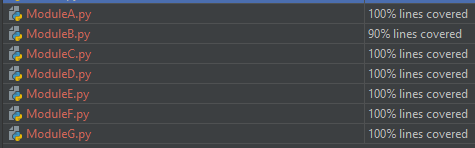
\includegraphics[width=0.8\textwidth]{Coverage1}
    \caption{Coverage report from top down testing.}
\end{figure}

\subsubsection*{Bottom up}
\footnotesize
\begin{centering}
\begin{tabularx}{\textwidth}{|q|q|X|q|}
    \caption{Test results resulting from the bottom up testing technique.} \\ \hline
    \textbf{Test ID} & \textbf{Module} & \textbf{Test Name} & \textbf{Pass} \\ \hline
    1   & TestModuleF   & test\_display\_data             & Yes \\ \hline
    2   & TestModuleG   & test\_data\_update              & Yes \\ \hline
    3   & TestModuleG   & test\_data\_update\_file\_error & Yes \\ \hline
    4   & TestModuleE   & test\_run\_exit                 & Yes \\ \hline
    \rowcolor[HTML]{FFB9B9}
    5   & TestModuleDFG & test\_delete\_data              & No  \\ \hline
    6   & TestModuleDFG & test\_getters                   & Yes \\ \hline
    7   & TestModuleDFG & test\_insert\_data              & Yes \\ \hline
    8   & TestModuleDFG & test\_setters                   & Yes \\ \hline
    \rowcolor[HTML]{FFB9B9}
    9   & TestModuleDFG & test\_update\_data              & No  \\ \hline
    10  & TestModuleCF  & test\_get\_f                    & Yes \\ \hline
    11  & TestModuleCF  & test\_set\_f                    & Yes \\ \hline
    12  & TestModuleCF  & test\_sort\_data                & Yes \\ \hline
    \rowcolor[HTML]{FFB9B9}
    13  & TestModuleBF  & test\_file\_not\_found\_error   & No  \\ \hline
    14  & TestModuleBF  & test\_get\_f                    & Yes \\ \hline
    15  & TestModuleBF  & test\_io\_error                 & Yes \\ \hline
    16  & TestModuleBF  & test\_load\_file                & Yes \\ \hline
    17  & TestModuleBF  & test\_set\_f                    & Yes \\ \hline
    18  & TestModuleA   & test\_add                       & Yes \\ \hline
    19  & TestModuleA   & test\_commands\_index\_error    & Yes \\ \hline
    20  & TestModuleA   & test\_commands\_no\_file        & Yes \\ \hline
    21  & TestModuleA   & test\_delete                    & Yes \\ \hline
    22  & TestModuleA   & test\_display\_help             & Yes \\ \hline
    23  & TestModuleA   & test\_empty\_command            & Yes \\ \hline
    24  & TestModuleA   & test\_exit                      & Yes \\ \hline
    25  & TestModuleA   & test\_get\_data                 & Yes \\ \hline
    26  & TestModuleA   & test\_help                      & Yes \\ \hline
    27  & TestModuleA   & test\_invalid\_command          & Yes \\ \hline
    28  & TestModuleA   & test\_load                      & Yes \\ \hline
    29  & TestModuleA   & test\_set\_data                 & Yes \\ \hline
    30  & TestModuleA   & test\_sort                      & Yes \\ \hline
    31  & TestModuleA   & test\_update                    & Yes \\ \hline
\end{tabularx}
\end{centering}
\normalsize

An image of the coverage report is provided below.
\begin{figure}[H]
    \centering
    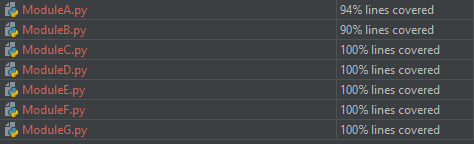
\includegraphics[width=0.8\textwidth]{Coverage2}
    \caption{Coverage report from bottom up testing.}
\end{figure}


\subsubsection*{Failed test case discussion}
\begin{itemize}
    \item Test ``test\_delete\_data'' (test 20 from top down, test 5 from bottom up): in this test, we attempted to trigger a \lstinline{FileNotFoundError} by having our program attempt to use a file that doesn't exist in the directory. However, as mentioned previously, the line of code that handles this specific exception is not reachable as the error is caught by an earlier exception that is a superclass of the \lstinline{FileNotFoundError} error. In order to fix this error, we could move this statement above the other statement like this:
    \begin{lstlisting}[language=Python, style=style]
        except FileNotFoundError:
            msg = "FileNotFoundError"
            print(msg)
        except IOError as e:
            print("Could not read file:{0.filename}".format(e))
    \end{lstlisting}
    \item Test ``test\_update\_data'' (test 29 from top down, test 9 from bottom up): in this test, we attempted to test updating a data entry. Due to the ambiguous nature of this function, the tester must make a judgement as to what it is supposed to do due to the lack of comments. Is it supposed to remove based on the printed list's index, or the index of an array where the first element is element 0? For my test, I assumed the former (i.e., attempting to remove index 2 would remove the 2nd item in the list). However, the test case fails in this case: attempting to remove the 2nd item ends up removing the 4th item (or the item at the 3rd index). In any case, this behavior is probably incorrect. A fix would be to change the indexing in the \lstinline{updateData} function in \lstinline{ModuleD.py} as follows:
    \begin{lstlisting}[language=Python, style=style]
        data[index - 1] = Entry(name, number)
        self.f.displayData(data)
        self.g.updateData(filename, data);
        return data
    \end{lstlisting}
    \item Test ``test\_file\_not\_found\_error'' (test 21 from top down, test 13 from bottom up): in this test, we attempted to test removing a data entry. Similarly to test 43, due to the lack of comments, we are left guessing as to what the correct behavior of this function is. Again, we will assume we are supposed to remove based on the printed list's index. This test case fails, however, as attempting to remove the $i$th element actually removes the $i+1$th element. A fix would be to change the indexing in the \lstinline{deleteData} function in \lstinline{ModuleD.py} as follows:
    \begin{lstlisting}[language=Python, style=style]
        del data[index - 1]
        self.f.displayData(data)
        self.g.updateData(filename, data)
        return data
    \end{lstlisting}
\end{itemize}

\subsection*{Q4 Discussion}
\begin{enumerate}
    \item As we saw from our testing, module isolation is effective at detecting hidden errors that may go unseen just from testing the entire system. For example, while updating and deleting from the database appear to work when the whole program is tested, the individual modules have errors. By coincidence, these errors cancel each other out when the whole program is tested, but it isn't always the case that errors will cancel each other out. 
    \item Top down testing is great when the most important code is in higher level modules. However, bottom up testing is more effective when the important code is in the lower level modules. Bottom up testing is also better for object oriented systems whereas top down testing is better for procedural oriented systems. Bottom up testing is also better if the system is to be built from the lower levels and up. 
    \item While integration testing is effective at testing the system as a whole, it does not scale well. As more modules are added, both bottom up and top down testing techniques require more and more effort. Both techniques will require more set up and tests. Bottom up will require more drivers. Top down will require the creation of more stubs.
    \item Stubs and drivers are effective ways of isolating the functionality of modules during testing. They allow for easy testing of modules that depend on other modules and are essential for any type of integration testing.
    \item In the modern world, systems are typically designed around the object oriented programming paradigm. As such, I believe bottom up integration testing is the most effective. As discussed earlier, bottom up testing is effective for object oriented systems as it allows easier testing of the low level modules (which are the modules that contain the important code in object oriented systems).
    \item I believe the bottom up testing technique would be the best for test driven development. This allows the lower level modules (which don't depend on anything) to be implemented first, then allows us to work up after the lower level modules are completed. This allows the verification of modules as we continue development.
    \item For testing software libraries, I believe the big bang integration testing technique would be the best choice. Typically, users are not be expected to test libraries; rather, the libraries should be tested by the developers of the library and then the user's system should be tested using the library. As such, it would make more sense to test the library and the user's code separately, then test the user's code combined with the library.
    \item I believe the bottom up technique would be easiest to maintain. While all techniques would require substantial effort to maintain, bottom up allows for a gradual build up of tests as low level modules don't depend on other modules. Bottom up also doesn't require the creation of stubs, which are typically harder to create than drivers.
    \item As we saw, we were able to effectively uncover some errors in our program by using incremental testing techniques. This type of testing can be somewhat effective for large projects, as it not only ensures individual modules are working but also makes sure that all modules are working harmoniously together. After all, it is possible for all individual modules of a system to be working while the program as a whole doesn't work at all. However, it may be impossible in practice for large projects due to the amount of tedious work required to get it set up. 
\end{enumerate}

\section*{Conclusion}
The purpose of this lab was to introduce integration white box testing techniques, namely, bottom up and top down testing techniques. We used Python and Python unittest to gain experience with integration testing.

Integration testing is the logical extension of unit testing. In this lab, we focused on incremental testing (top down and bottom up). Incremental testing is where the set of previously tested modules are combined with the next module to be tested before running tests. There are two common types of incremental testing:
\begin{itemize}
    \item Bottom up: where the lowest level modules are tested in isolation, then higher level modules are added incrementally, and
    \item Top down: where the highest level modules are tested in isolation (stubbing lower level modules), then lower level modules are added incrementally.
\end{itemize}
For bottom up testing, lower level modules typically don't function by themselves. As a result, we need driver code to test these lower level modules. For top down testing, in order to just test a higher level module that may depend on lower level modules, we use stubs. Stubs mock the functionality of lower level modules so that the higher level module can be tested in isolation. Stubs return dummy values or makes an assertion so that the higher level modules can still run and be tested. 

In the lab, we tested a simple database system that had seven modules, Module A to module F. 
\begin{itemize}
    \item For bottom up, we created drivers for the lowest level modules. We then created drivers for the middle level modules, then finally, a driver for the top level module. These drivers ran tests. We found three failed test cases.
    \item For top down, we started at the top level module and stubbed the behavior of the middle level modules. We then tested the middle level modules where the lower level modules were stubbed. Lastly, we tested the system as a whole with nothing stubbed. We also found three failed test cases.
\end{itemize}

Through both types of incremental testing (top down and bottom up), we were able to discover three errors: there were some errors when indexing the database for updates and deletion and there were areas of code that were unreachable. We investigated these failed test cases and proposed fixes to fix these test cases. We saw that incremental testing is an effective way to test a program, but comes at the cost of requiring a lot of tedious work to complete. 

\end{document}
